\chapter{Arhitectura sistemului}

În acest capitol vom construi arhitectura sistemului, astfel încât aceasta să își atingă scopul precizat anterior, ținând cont de proprietățile enumerate pe care soluția trebuie să le aibă. Pentru o descriere mai amplă și mai organizată a arhitecturii vom apela la metologiile clasice folosite în dezvoltarea arhitecturilor software.

\section{Părțile implicate}

Părțile implicate, sau \textit{stakeholderii} cum mai sunt denumite acestea în literatură, sunt în număr de 3. Avem astfel dezvoltatorul sistemului de experimentare, clientul serviciului (dezvoltatorul aplicației principale) și utilizatorul final al aplicației principale. Ne vom concentra în cele ce urmează pe ultimele două părți.

\textbf{\textit{Clientul sistemului}} este reprezentat de dezvoltatorul produsului ce necesită efectuarea experimentelor. Acesta dorește să poată folosi cât mai ușor sistemul de experimentare, prin intermediul unui număr cât mai mare de limbaje de programare. Interesul acestuia este ca serviciul pe care lucrarea îl propune să fie cât mai flexibil și extensibil, pentru a oferi acestuia posibilitatea de a fructifica cât mai multe oportunități, evitând adăugarea complexității suplimentare aplicației inițiale, prin gestionarea experimentelor în codul acesteia.

\textbf{\textit{Utilizatorul final}} este cel căruia i se adresează produsul software principal dezvoltat. Acesta dorește ca aplicația să poată răspunde foarte rapid comenzilor acestuia, iar asta lucru înseamna că serviciul pe care lucrarea îl propune nu trebuie să reprezinte un \textit{bottleneck}\footnote{O componentă ce încetinește întreg sistemul} pentru întreaga aplicație.

\subsection{Perspectiva funcțională}

Având părțile implicate definite, vom trece mai departe să conturăm perspectiva funcțională a fiecăreia dintre acestea.

\textbf{\textit{Clientul sistemului}} va dori să poată să gestioneze lista experimentelor, prin adăugare și ștergere, și să poată vizualiza lista cu cele disponibile. Va putea de asemenea să definească valorile variabilelor din cadrul unui experiment. Pe lângă aceste aspecte, în codul aplicației principale va dori să se efectueze un apel, având ca parametrii identificatorul experimentului și identificatorul entității, iar mai apoi să obțină toți parameterii variabilelor, \textit{pentru toate experimentele} în care entitate respectivă se va regăsi.

\begin{remark}
	Deși există sisteme de experimentare ce oferă posibilitatea editării parameterilor unui experiment, lucrarea consideră această abordare defectuoasă, deoarece astfel de operații pot invalida rezultatele finale. De aceea vom considera definiția unui experiment ca o valoare \textbf{imutabilă}\footnote{Toți parameterii vor avea valori constante, ce nu pot fi modificate}. 
\end{remark}

\textbf{\textbf{Utilizatorul final}}, este cel care va fi inclus în anumite experimente, și de aceea dorește ca experiența sa să fie una cât mai uniformă în cadrul aplicației principale. De exemplu, dacă se testează eficiența dispunerii unui anumit buton în cadrul unei aplicații, clientul va dori să vadă, la fiecare vizită, butonul în aceeași poziție. De altfel, dacă acesta ar observa dispuneri diferite, rezultă ca elementele eșantionului nu au fost identic și independent distribuite. Din acest lucru reiese ca sistemul de experimentare va trebui să asocieze în mod consistent o entitate în cadrul aceluiași grup dintr-un experiment. 

\section{Calități arhitecturale de sistem}

Vom prezenta în cele ce urmează calitățile arhitecturale de sistem, importante pentru serviciul pe care dorim să îl dezvoltăm. În același timp vom menționa tacticile și stilurile arhitecturale pe care le vom utiliza pentru a reuși implementarea aceste calități.

\textbf{\textit{Adaptabilitatea}} este una din cele mai importante calități arhitecturale de sistem pentru un serviciu de experimentare. După cum am argumentat, considerăm vitală posibilitatea de a adăuga funcționalități, într-un mod facil și rapid, la sistemul dezvoltat, fiecare client al aplicație având nevoi diferite.

Pentru a putea îndeplini această calitate arhitecturală, vom folosi o serie de diverse tactici. Prima este aceea de a efectua o abstractizare a modulelor sistemului astfel încât să existe \textit{cât mai puține dependențe} între acestea. De asemenea vom folosi \textit{coerența semantică}, prin care fiecare modul va avea o funcționalitatea bine definită, iar relațiile între acestea vor fi definite riguros. Astfel, de fiecare dată când vom executa o modificare vom putea identifica toate modulele ce necesită modificări.

\textbf{\textit{Disponibilitatea}} este o altă calitate arhitecturală importantă. În orice aplicație modernă, experimetarea constituie un element primordial, aceasta regăsindu-se atât pe partea de \textit{frontend}, prin testarea diferitelor interfețe, cât și pe partea de \textit{backend}, prin compararea performanței algoritmilor. De aceea trebuie ca serviciul de experimentare să fie disponibil pe o durată cât mai îndelugată de timp, și să se limiteze  perioada de \textit{downtime}\footnote{Durata de timp în care sistemul nu este disponibil.}.

Tactica pe care o vom folosi este aceea de a dezvolta o \textit{arhitectură distribuită}, astfel încât să evităm existentă unui \textit{single point of failure}\footnote{O componentă a sistemului care în caz de eroare compromite întreg sistemul}. Detectarea erorilor se va face folosind o tactică de tipul \textit{heartbeat}, în care vom verifica periodic starea unei componente a sistemului. Astfel, fiecare modul al aplicației, identificat anterior, în cazul în care nu va funcționa corect, nu va compromite întreg sistemul, deoarece responsabilitățile acestuia vor fi preluate de un alt modul identic ce va rula în paralel într-un alt mediu.

\textbf{\textit{Scalabilitatea}} sistemului este esențială. Ne dorim ca produsul să poată fi folosit atât de companii mici, \textit{start-up-uri}, dar și de companii mai mari, iar acest lucru presupune posibilitatea de a rula sistemul pe o gamă variată de resurse. Prin rularea distribuită, vom putea scala sistemul pe orizontală, prin simpla adăugarea a mai multor servere, evitând scalarea pe verticală, ce presupune mărirea resurselor mașinilor pe care este rulată aplicația, fiind cunoscut faptul că astfel de investiții sunt substanțiale, și greu de implementat.

\textbf{\textit{Performanța}} este una din calitățile arhitecturale asupra căreia trebuie să acordăm atenție. Pentru a obține o \textit{performanță} cât mai bună, vom folosi tactica gestionării resurselor, introducând \textit{concurența} în interiorul sistemului. Având în vedere faptul că vom avea foarte multe cereri către sistem, ce vor trebui rezolvate în același timp, este natural să urmăm o astfel de tactică. Nu în ultimul rând, concurența este ușor de modelat, și în funcție de mediul în care rulează serviciul poate implica paralelism.

\section{Stilul arhitectural}

Pentru a putea îndeplini toate calitățile arhitecturale enumerate anterior, vom examina o suită de \textit{stiluri arhitecturale}, pentru a putea observa care dintre acestea este cel mai potrivit pentru un sistem de experimentare. În mod evident, stilurile arhitecturale de tipul \textit{data-flow} sau \textit{batch-processing} nu se pliază cerințelor sistemului, deoarece experimentele trebuie să poată fi adăugate sau șterse cu ușurință, oferind o velocitate de dezvoltare crescută. Este de remarcat faptul că un sistem de tipul client-server este cel mai indicat pentru a fi folosit în situația de față, având în vedere modul în care va fi utilizat serviciul. Cu toate acestea, după cum am menționat anterior, dorim să oferim posibilitatea clienților de a extinde foarte ușor sistemul de experimentare, pentru a-l particulariza conform cerințelor acestora. Acest lucru însă nu este trivial de realizat, mai ales în condițiile în care aplicație este dezvoltată sub forma unui \textit{monolit}.

Calitățile arhitecturale expuse, dar și scopul sistemului, ne îndrumă către o arhitectură bazată pe \textbf{servicii\textit{}}. In mod imediat, abordarea clasică pe care o putem urma este aceea de \textit{SOA}\footnote{Service Oriented Architecture - Arhitectură orientată pe servicii}. Acest tip de arhitectură are însă dezavantajul de a fi de complexă, iar în final modulele componente nu devin independente, ci \textit{autonome}. Orice aplicație de de tip \textit{SOA} este gestionată și distribuită asemeni unui \textit{monolit}. De aceea, lucrarea propune o abordare arhitecturală mai nouă, bazată pe \textbf{\textit{microservicii}}.\cite{buildingmicro} 

\subsection{Arhitectura bazată pe microservicii}

Arhitecturile bazate pe \textit{microservicii} reprezintă un nou mod de abordare a aplicațiilor, care se diferențiază segmentarea fiecărui modul al aplicației într-un serviciu independent. Aceste servicii pot comunica prin intermediul unui mecanism ce presupune un \textit{overhead} minimal, iar de obicei acest mecanism folosit este protocolul HTTP\cite{onmicro}. Motivația principală ce stă la baza acestui tip de arhitectură constă în posibilitatea de a pune în producție fiecare dintre aceste servicii \textbf{independent} de celelalte, iar acest fapt rezultă într-o viteză crescută de dezvoltare.

\begin{definition}
	Un microserviciu reprezintă un proces, ce are un \textbf{scop singular}, și care comunică cu alte microservicii prin intermediul unui protocol bine definit.
\end{definition}

Unul din motivele pentru care microserviciile au reușit să fie adoptate de un număr relativ mare de companii, printre care menționăm \textit{Google}, \textit{Amazon} și \textit{Netflix}, într-un timp atât de scurt, se datorează apariției tehnologiilor noi precum \textit{Docker}, ce permit rularea unei aplicații în interiorul unui \textit{container}, complet izolat de restul aplicațiilor de pe aceeași mașină. Prin container înțelegem un strat de abstractizare, superior din punctul de vedere al performanței față de mașinile virtuale. Astfel un \textit{container} încapsulează toate dependențele necesare unei aplicații, dar împarte același \textit{kernel} al sistemului de operare cu restul containerelor. Putem rula în acest mod o serie întreagă de microservicii, fiecare în interiorul containerului său, independent de restul sistemului.

\subsubsection{Avantaje}

Spre deosebire de aplicațiile clasice, de tip monolit, astfel de aplicații distribuite au un avantaj foarte interesant, ce provine din faptul că fiecare serviciu component al său poate fi scris în orice limbaj de programare, atât timp cât poate efectua comunicarea cu restul serviciilor, prin intermediul protocolului ales. Ca o consecință naturală, acest fapt oferă o flexibilitate mult mai mare dezvoltatorilor, conferind libertatea de a alege mult mai ușor tehnologie potrivită, ce se pliază problemei particulare pe care dorește să o rezolve serviciul. Implicit, prin fragmentarea aplicației se pot efectua mult mai ușor și tranzițiile către alte tehnologii, lucru ce este foarte greu, sau de mult ori imposibil de efectuat în contextul unei aplicații monolotice. În cazul clasic, se folosește aceeași tehnologie pentru întregul sistem, un dezavantaj major.

Un alt beneficiu este acela de a avea ușurința de scalare rapidă a unei platforme bazată pe microservicii. Se pot optimiza resursele folosite de către sistem, prin rularea a multiple instanțe ale unui serviciu, în spatele unui \textit{load-balancer}. Cum aplicațiile moderne rulează în \textit{cloud}, se pot adăuga sau elimina instanțe extrem de rapid, în mod programatic. Din nou se poate observa cum fracționarea sistemului conduce către o flexibilitate sporită, pe care o aplicație clasică nu o poate oferi. Posibilitatea de a scala doar componentele necesare reduc costul de rulare a aplicației.

Compunerea serviciilor este un alt aspect interesant, ce este facilitat de acest tip de arhitectură. De exemplu, tot mai multe aplicații trebuie să ofere o experiența unitară, pe mai multe platforme, ce permite utilizatorilor să schimbe dispozitivul în mijlocul unei sesiuni de lucru. Prin segmentarea corectă a aplicației se vor putea compune serviciile pentru a reutiliza datele oferite de serviciile generale, în timp ce va exista posibilitatea de dezvoltare a unor instanțe specializate pentru tipuri particulare de platforme. 

Nu în ultimul rând trebuie amintită viteza de dezvoltare și de punere în producție a sistemului, ce este cu mult superioară față de aplicațiile clasice, monolitice. După cum am prezentat anterior, fiecare serviciu este dezvoltat și lansat în mod independent fața de celelalte. Se oferă posibilitatea de a scala dezvoltarea aplicației prin descentralizarea acesteia. Fiecare serviciu nu va depinde de celelalte, iar acest fapt îmbunătățește efectele pe care le au diferite concepte. De exemplu integrarea continuă este mult mai ușor și sigur de folosit în același timp, deoarece pentru a lansa o componentă se vor efectua doar testele necesare acesteia. 

\subsubsection{Dezavantaje}

Desigur, pe lângă avantajele evidente, menționate anterior, există și o serie de dezavantaje pe care arhitectura bazată pe microservicii le prezintă\cite{onmicro}. Primul dezavantaj evident este acela al complexitații necesare punerii în producție a fiecărui serviciu, în mod individual, și orchestarea tuturor serviciilor ca un ansamblu. Există însă o întreagă suită de servicii ce orchestrare ce vin în ajutorul dezvoltatorilor pentru a putea minimiza această complexitate, precum \textit{Kubernetes}, dezvoltată de \textit{Google}. Se permite astfel, prin introducerea unui strat de abstractizare a sistemului, gestionarea fluentă și corectă a întregului serviciu. \cite{kubernetes}

De altfel, complexitatea crescută a sistemelor distribuite, de care un dezvoltatorii trebuie să țină cont, reprezintă un dezavantaj a arhitecturii bazate pe microservicii, în ceea ce privește ușurința de dezvoltare. 

Deși împărțirea aplicației în microservicii duce la ușurarea procesului de testare a fiecărui serviciu, apare o altă problemă și anume aceea a efecutării testării \textit{end-to-end}, sau de integrare, a întregului sistem. 

\begin{remark}
	O capcană pe care o prezintă arhitectura bazată pe microservicii este aceea a dezvoltării unui număr prea mare de microservicii, prea specializate, ce poartă numele de \textbf{nanoservicii}, iar această practică este descurajată.
\end{remark}

Un ultim dezvatantaj, este reprezentat de durata de comunicare în rețea între microservicii. Cu toate acestea, de multe ori vom rula întreg sistemul în cadrul aceluiași \textit{data-center}, iar rețelele au ajuns la o performanță considerabilă în astfel de situații. Menționăm că în cazul în care sistemul dorește să efectueze procesări masive de date, \textit{big data}, folosirea unei astfel de arhitecturi este puternic descurajată, însă serviciul pe care îl vom propune nu se încadrează în această categorie.

\subsubsection{Concluzie}

Deși prezintă o serie de dezavantaje, lucrarea consideră că stilul arhitectural bazat pe \textit{microservicii} se pliază cel mai bine pentru un sistem de experimentare. Flexibilitatea și extensibilitatea sporită ce sunt oferite de o astfel de arhitectură fața de cele tradiționale, recomandă acest stil arhitectural.

\section{Principii arhitecturale}

Secțiunea anterioară a justificat motivele utilizării unei arhitecturi bazate pe microservicii. În cele ce urmează următoare vom defini un set de principii pe care le vom adopta în dezvoltarea sistemului, împreună cu motivația pentru alegerea acestora. Prin stabilirea principiilor, ne vom facilita misiunea de a segmenta serviciul de experimentare, indentificând modulele componente, acest pas fiind cel mai important și totodată dificil, în elaborarea arhitecturii.

\subsubsection{Servicii \textit{stateless}}

Vom impune o regulă generală, și anume ca toate serviciile să fie considerate \textit{stateless}. Prin acest lucru înțelegem că acestea nu vor încapsula informații legate la starea aplicației. Astfel, în mod teoretic, scalarea serviciului pe orizontală se poate face prin simpla adăugare sau eliminare a mai unor instanțe ale acestuia. Aceast principiu, sugerează REST ca și protocol de comunicare între servicii, de altfel acesta fiind protocolul folosit cel mai des în acest tip de arhitectură\cite{buildingmicro}. 

\subsubsection{Separarea datelor}

Principiul separării datelor sugerează ca fiecare microserviciu să își gestioneze datele prin folosirea unei baze de date proprii. Astfel, fiecare serviciu va alege tipul de bază de date care este cel mai potrivit pentru acesta. De exemplu un serviciu ce permite operații CRUD \textit{(create, read, updated, delete)} va folosi un RDBMS \textit{(Relational Database Management System)}, în timp ce un serviciu de autenficare poate utiliza o bază de date No-SQL. 

Motivul principal pentru implementarea ideilor formulate de acest principiu, este acela că folosirea unei baze date date comune ar duce la dependențe între microservicii, provocate de folosirea comună a aceleași schema a bazei de date. Astfel, daca un serviciu solicită modificarea schemi, restul serviciilor care o folosesc vor trebui să fie actualizate, și astfel pierdem din flexibilitatea arhitecturii. Pe de altă parte există posibilitatea de a avea inconsistențe între diferitele baze de date. Pentru soluționarea acestei probleme există așa numitele unelte \textit{Master Data Management}. Acestea efectuează verificări periodice și oferă alerte administratorilor de sistem, și sincronizează bazele de date.

\subsubsection{Asocierea serviciu-\textit{container}}

În ceea ce privește modul de rulare a sistemului, există câteva abordări posibile. Prima dintre acestea este maparea unui serviciu pe o mașină. Este evident că această strategie este una costisitoare, și nefezabilă pentru companiile mici. O altă soluție are la bază maparea unui serviciu pe o mașină virtuală, dar și această abordare este defectuoasă, deoarece gestionarea mașinilor virtuale reprezintă un proces complex și complicat. În final, vom apela la strategia ce presupune maparea unui serviciu în interiorul unui container de Linux, precum \textit{Docker}. Astfel, vom putea multiplexa multiple servicii pe un număr limitat de mașini prin intermediul unor unelte de orchestrare, cum ar fi \textit{Kubernetes}. Această ultimă abordare este cea mai "curată", oferind serviciilor independența necesară.

\subsubsection{Expunerea unui API}

Din cauza faptului că arhitectura cu microservicii este foarte flexibilă, pot apărea dificultăți în gestionarea comunicării clientului cu sistemul. Fiecare apel trebuie să fie făcut către serviciul corespunzător. Gestionarea unor astfel de apeluri însă nu este recomandată să aibă loc pe partea de client.  Pentru acesta este ideală comunicarea simplă sub forma unui API\footnote{Application Programming Interface} comun, pentru întreaga aplicație. Soluționarea acestor probleme vine prin adăugarea unei alte componente și anume un \textit{API Gateway} sau un \textit{Reverse Proxy}. Clientul va face astfel mereu apelul către această componentă, care va ruta cererea mai departe serviciului corespunzător. Dezavantajul este acela că se adaugă complexitatea a încă unei componente la sistem, dar lucrarea consideră acest \textit{trade-off} benefic. 

\section{Dezvoltarea arhitecturii}

În această secțiune vom descrie și vom construi gradual arhitectura sistemului de experimentare pe care lucrarea îl propune, conformându-ne principiilor enunțate anterior.

\subsection{Identificarea serviciilor}

Vom începe natural pentru arhitectura aleasă, indentificând componentele sistemului. După cum am descris anterior, clientul sistemului de experimentare dorește să poată gestiona rapid adăugarea și ștergerea experimentelor. Astfel, conform principiului de separare a datelor, putem identifica un prim microserviciu, acela de \textbf{\textit{Repository}}, sau \textit{Magazie} a experimentelor. Responsabilitatea acestei componente va fi gestionarea experimentelor, utilizând o bază de date proprie.

Pe lângă componenta identificată deja, este absolut necesar un mecanism de asignare a unei entități către un experiment. O primă idee, intuitivă, spune că putem avea o componentă care va interoga magazia experimentelor și efectua apoi toate sarcinile necesare. Dar, deoarece știm ca dorim să experimentăm, cu mai multe astfel de modalități de asignare a entităților către experimente, și dorim de asemenea ca și clientul aplicației să poată folosi orice abordare dorește, vom construi o componentă separată ce se va ocupa doar de acest aspect, pe care o vom numi \textit{\textbf{Assigner}}, sau \textbf{\textit{Serviciu de atribuire}}. Acest serviciu se va ocupa exclusiv de gestionarea apartenenței unei entități la unui grup din cadrul unui experiment descris.

Ne amintim că, din perspectiva funcțională a clientului final, acesta dorește ca experiența sa să fie cât mai uniformă. Acestă doleanță se traduce prin asignarea, de fiecare dată, a unei entități către aceleași grupuri din anumite experimente. Efectul poate fi obținut prin construcția unui \textit{Assigner} ce este determinist. Dar, având în vedere că nu putem forța acest comporatament componentei respective, va trebui să construim o altă componentă, care să stocheze informații referitoare la asignarea inițială a unui utilizator, pe care o vom numi \textit{\textbf{Store}} sau \textbf{\textit{Depozit}}. Astfel, dacă o entitate a fost deja asignată unui grup, va trebui ca sistemul de experimentare să garanteze că a doua oară când va fi interogat, pentru aceeași entitate, va oferi același răspuns.

\begin{remark}
	Dacă serviciul Assigner este determinist atunci nu este necesară existența serviciului Store. 
\end{remark}

Nu în ultimul rând, avem nevoie de un serviciu care să coordoneze si să orchestreze interacțiunile între cele trei servicii descrise, acesta fiind punctul ce va expune un \textit{API} pentru clientul aplicației. Vom denumi acest serviciu \textit{\textbf{Experimento}}, acesta luând numele framework-ului de experimente pe care lucrarea îl propune. 

Am indentificat deci 4 microservicii ce vor fi nelipisite din alcătuirea sistemului de bază. Le vom recapitula sumar, pentru a le putea vizualiza ușor.

\begin{itemize}
	\item \textbf{Repository:} Gestionează experimentele
	\item \textbf{Assigner:} Assignează o anumită entitate unui grup dintr-un experiment
	\item \textbf{Store:} Reține asignarea inițială a unui utilizator
	\item \textbf{Experimento:} Componenta principală, care expune \textit{API-ul} serviciului 
\end{itemize}

\begin{remark}
	Serviciul \textit{Experimento} reprezintă componenta centrală a sistemului, iar dezvoltarea corectă a acestuia este critică. Lucrarea va oferi un exemplu de implementare concretă.
\end{remark}



\subsection{Descrierea mesajelor}

Într-o arhiectură bazată pe microservicii este foarte importantă comunicarea ce se realizează între componente. Soluția naturală este aceea de a standardiza mesajele, și a comunica folosind un anumit format, bine definit, pentru a evita posibilele discrepanțe.

Deși există un număr mare de librării ce sunt folosite pentru serializarea și deserializarea mesjaelor, cât și pentru efectuarea de apeluri de tip \textit{RPC}\footnote{Remote procedure call}, precum \textit{Protocol Buffers}, \textit{Apache Thrift}, \textit{Message Pack}, \textit{Avro}, ș.a.m.d, toate acestea folosind un format binar, de multe ori alegerea \textit{de facto} este aceea a mesajelor de tip JSON, deoarece mesajele codificate folosind această notație sunt \textit{human-readable}.

În cele ce urmează vom încerca să definim mesajele pe care le vom folosi pentru comunicare într-un mod cât mai simplu, astfel încât să putem implementa această structură folosind oricare din bibliotecile menționate anterior. Sintaxa ce va fi folosită pentru a putea descrie mesajele este aceea oferită de \textit{IDL-ul}\footnote{Interface Definition Language} utilizat de către \textit{Protocol Buffers 3}. Menționăm faptul că folosirea unui astfel de protocol, aduce o serie întreagă de beneficii, pe care le vom discuta într-un capitol ulterior, legat de tehnologiile folosite.

\begin{remark}
	Reamintim că lucrarea nu consideră că mesajele trebuie să urmeze în mod neapărat această structură, ci doar o recomandă.
\end{remark}

Mesajul principal ce va sta la baza sistemului de experimentarea este acela ce va descrie complet un experiment. Va trebui să încapsulăm informații referitoare la experiment, variabilele, și grupurile acestuia, dar și să oferim posibilitatea de a integra alte informații auxiliare. Lucrarea propune următoarea strucutră pentru un astfel de mesaj:

\break

\begin{center}
	\begin{lstlisting}[language=proto3]
message Experiment {
	ExperimentInfo info = 1;
	map<string, VariableInfo> variables_info = 2;
	map<string, GroupInfo> groups_info = 3;
	
	map<string, string> whitelist = 4;
	
	// Incapsulare detalii auxiliare.
	google.protobuf.Any details = 100;
}
	\end{lstlisting}
\end{center}

Se identifică trei mesaje ce vor trebui definite: \textit{ExperimentInfo}, \textit{VariableInfo}, alături de \textit{GroupInfo}.

\begin{center}
	\begin{lstlisting}[language=proto3]
message ExperimentInfo {
	string id = 1;
	string seed_value = 2;
	double size = 3;
	int64 started = 4;
}
	\end{lstlisting}
\end{center}

Primul dintre acestea, și anume mesajul de tip \textbf{\textit{ExperimentInfo}} va fi folosit pentru a încapsula informații generale valabile legate de experimentul în cauză, precum identificatorul acestuia, data de start, ș.a.m.d.

\begin{remark}
	Câmpul \textbf{seed\_value} este folosit pentru a putea controla replicabilitatea rezultatelor unui experiment, în timp ce câmpul \textbf{size} va avea o valoare între 0 și 1, și va reprezenta partea entităților ce va lua parte la experiment.
\end{remark}

\begin{lstlisting}[language=proto3]
message VariableInfo {
	repeated string options = 1;
}
\end{lstlisting}

Vom exprima lista de posibile alegeri ale unei variabile ca un vector de șiruri de caractere, ce va fi conținut de mesajul \textbf{\textit{VariableInfo}}. Am ales această abordare, în detrimentul unor soluții mai complexe precum cea oferită de \textit{PlanOut}, deoarece ea este foarte simplă, și minimizează efortul necesar elaborării și înțelegerii unui experiment.

\begin{center}
	\begin{lstlisting}[language=proto3]
message GroupInfo {
	double initial_size = 1;
	map<string, string> variables = 2;
}
	\end{lstlisting}
\end{center}

În final, mesajul \textbf{\textit{GroupInfo}} va descrie caracteristicile fiecărui grup. Deoarece, imediat cum un experiment a fost adăugat, nu există informații \textit{a priori}, va trebui ca pentru un experiment, indiferent de ce \textit{Assigner} va fi folosit pentru acesta, să specifice dimensiunea de început a grupului, prin intermediul câmpului \textit{initial\_size}. Aceasta are rol orientativ, pentru a cunoaște modul de asignare a entităților către anumite experimenete, atunci când nu există alte informații. De asemenea, informația poate fi folosită și atunci când un assigner folosește un mecanism de tip \textit{holdout}, pentru a determina distribuția entităților ce fac parte din acesta. De aceea, va trebui ca suma acestui câmp, peste toate grupurile experimentului, să fie egală cu 1.

Câmpul \textit{Variables} asociează fiecărei variabile o anumită valoare pentru aceasta. Menționăm că trebuie efectuată verificarea în așa fel încât valoarea variabilei să fie validă, cu alte cuvinte să fie specificată anterior, în membrul \textit{options} al mesajului \textit{VariableInfo}, corespunzător grupului în cauză.

\break

\subsection{Definirea interfețelor}

Fiecare din microserviiciile identificate a fost descris, din punct de vedere funcțional, ilustrând rolul și cerințele acestuia. \textit{Framework}-ul pe care lucrarea dorește să îl dezvolte, propune o implementarea concretă pentru micro-serviciul \textit{Experimento}, unică. Pentru restul de trei microservicii indentificate, le vom descrie sub forma unor interfețe. Vom dezvolta mai apoi o serie de implmenetări concrete pentru acestea, în capitolul corespunzător dezvoltării aplicației. În definierea metodelor, ne vom folosi de mesajele definite anterior, pentru a putea descriere interfețele într-un mod consistent.

\begin{remark}
	Vom încerca să definim interfețele într-un mod cât mai minimal, pentru a putea oferi o flexibilitatea mare programatorului.
\end{remark}

\subsubsection{Repository}

Deși responsabilitatea principală a microserviciului \textit{Repository} este aceea de a gestiona experimentele, nu vom include în această interfața metode referitoare la aceste acțiuni. Motivul principal este acela de a oferi utilizatorilor serviciului flexibilitatea de a-și dezvolta propria modalitate de gestionare a experimentelor. Astfel, singura metodă pe care interfața \textit{Repository} va trebui să o implementeze este aceea care oferă lista tuturor experimentelor active. Motivul este acela că microserviciul \textit{Experimento} va avea nevoie de aceasta pentru a putea întoarce valorile variabilelor pentru toate experimentele unei entități. Dorim această abordare de a obține toate valorile experimentelor în \textit{batch} pentru a putea evita suprasolicitarea serviciului de experimentare. Rămâne astfel datoria serviciului principal să reactualizeze în mod regulat lista cu experimentele.

\begin{center}
	\begin{lstlisting}[language=proto3]
type Repository interface {
   GetExperiments() (map[string]Description, serror)
}
	\end{lstlisting}
\end{center}

\begin{remark}
	Metoda \textit{GetExperiements} trebuie să fie \textbf{thread-safe}\footnote{Să poată fi accesată simultan de mai multe thread-uri}, din cauza naturii concurente a întregului sistem.
\end{remark}

În cazul în care nu a putut fi obținută lista experimentelor active, este necesar ca metoda să întoarcă o eroare, pentru a semnala componentei centrale \textit{Experimento} acest aspect. Ea va prelua apoi responsabilitatea gestionării erorii.

\subsubsection{Store}

Cum microserviciul \textit{Store} este responsabil pentru a reține asignarea unei entități către un experiment, vom expune două metode ale interfeței, una pentru a seta alegerea inițiala și alta pentru a interoga existența unei astfel de alegeri. Acestea vor trebui să primească ca parametru identificatorul entintății, și identificatorul experimentului, iar cea de \textit{set}, pe lângă acestea va primi ca parametru și identificatorul grupului unde a fost asignată entitatea.

\begin{center}
	\begin{lstlisting}[language=proto3]
type Store interface {
   SetExperimentGroup(entityID, expID, group string) error
   GetExperimentGroup(entityID, expID string) (string, error)
}
	\end{lstlisting}
\end{center}

\subsubsection{Assigner}

Microserviciul \textit{Assigner} este foarte important, deoarece diferite implementări ale acestuia vor rezulta în diferite comportamente ale sistemului de experimentare. Vom folosi o singură metodă în această interfață ce va primi ca parametrii identificatorul entității, iar mai apoi întreaga descriere a unui experiment. Metoda va returna un șir de caractere ce va corespunde id-ului unui grup din cadrul experimentului, acest fiind grupul către care entitatea va fi asignată.

\begin{center}
	\begin{lstlisting}[language=proto3]
type Assigner interface {
  AssignGroup(entityID string, e Experiment) (string, error)
}
	\end{lstlisting}
\end{center}

\begin{remark}
	Metoda \textbf{AssignGroup} nu trebuie să fie determinstă, dar aceasta trebuie să fie thread-safe.
\end{remark}

\subsubsection{Experimento}

Deși serviciul \textit{Experimento}, după cum am precizat anterior, nu va fi implementat prin intermediul unei interfețe, vom descrie interogările pe care un client le poate face către acest serviciu, fie printr-un mecanism de tip \textit{REST} sau \textit{RPC}, cu ajutorul următorei signaturi:

\begin{center}
	\begin{lstlisting}[language=proto3]
func GetAllVariables(entityID string) (AllVariables, error)
func GetVariables(expID, entityID string) (Variables, error)
	\end{lstlisting}
\end{center}

După cum se poate observa, vom expune posibilitatea de a interoga variabilele tuturor experimentelor din care face parte un utilizator.

\begin{remark}
	Lucrarea sugerează utilizarea unui mecanism de caching în aplicația centrală, pentru a evita supraîncarcarea serviciului \textit{Experimento}.
\end{remark}

\subsection{Îmbunătățirea performanțelor}

După cum am văzut, arhitectura serviciul este construită pentru a facilita scalarea sistemului pe orizontală. Putem însă îmbunătăți performanța serviciul, printr-un mecanism eficient de gestionare a resurselor. Acest lucru se poate obține fie prin introducerea paralelismului în sistem, fie prin introducerea concurenței în sistem. 

Sistemele bazate pe o arhitectură cu microservicii, au o natură concurentă, cauzată de multiplele comunicări ce trebuie efectuate între servicii. Acest aspect, coraborat cu natura dinamică a unui serviciu de experimentare, ce presupune operații de gestionare a experimentelor, executate simultan cu operații de interogare a variabilelor, ne indică mecanismul pe care îl putem utiliza. De aceea vom introduce \textbf{concurența} în serviciul pe care îl vom dezvolta. Mecanismul de concurență pe care îl vom folosi este acela implementat de limbajul de programare \textit{Go}, și este inspirat de către lucrarea \textit{Communicating Sequential Processing}\cite{hoare_csp}. De aceea, algoritmii pentru un microserviciu vor folosi mecanisme precum \textit{canale} pentru a implementa concurența.

\subsection{Arhitectura finală}

În această secțiune am reușit să descriem principiile arhitecturale pe care le vom urmări, alături de motivația acestora, pentru ca mai apoi să indetificăm microserviciile și modul de utilizare al acestora. Se poate observa din descrierea componenelor că microserviciul \textit{Experimento} este componenta centrală a serviciului; aceasta comunică cu restul microserviciilor. Dar, pe lângă aceste interacțiuni, vor mai exista cereri efectuate de către utilizatorii sistemului de experimentare pentru a gestiona lista experimentelor. 

Aceste interacțiune, pot conduce la multiple probleme ce pot apărea, dar pe care le putem rezolva folosind un \textit{API Gateway}. Vom vizualiza arhitectura componentelor cu ajutorul unei diagrame de tip UML, prezentate în figura \ref{fig:components}. Se poate observa cum, prin definirea interfețelor, obținem o arhitectură simplă, ușor de înțeles.

\begin{figure}[H]
	\centering
	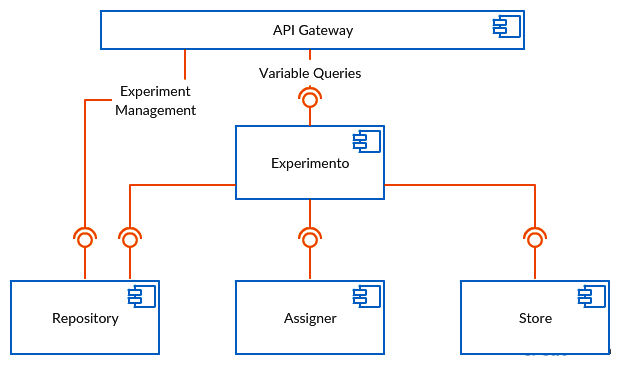
\includegraphics[max width=14cm,keepaspectratio]{components}
	\caption{Diagrama pentru modul de procesare a unei cereri}
	\label{fig:components}
\end{figure}

\begin{remark}
	Fiecare componentă din figura \ref{fig:components} va rula în mai multe instanțe, pentru a introduce redudanță, astfel încât funcționarea greșită a unei componente să nu afecteze întreg sistemul.
\end{remark}  

Pentru a exemplifca modul în care sistemul de experimentare, dar și pentru a ilustra cum comunică componenta centrală a acestuia, cu restul microserviciilor, vom reprezenta grafic procesul ce are loc atunci când serviciul este interogat. 

Menționăm faptul că alte facilități pe care sistemul le va implementa, precum adăugarea și eliminarea de servicii sunt triviale, și de aceea ne vom concentra atenția asupra acestui aspect, eliminând de asemenea din diagramă, componenta ce reprezintă \textit{API Gateway}. Vom folosi o diagramă UML \footnote{Unified Modelling Language} de tip secvențial, ce ne va permite să ilustrăm facil comunicarea. 

\begin{figure}[H]
	\centering
	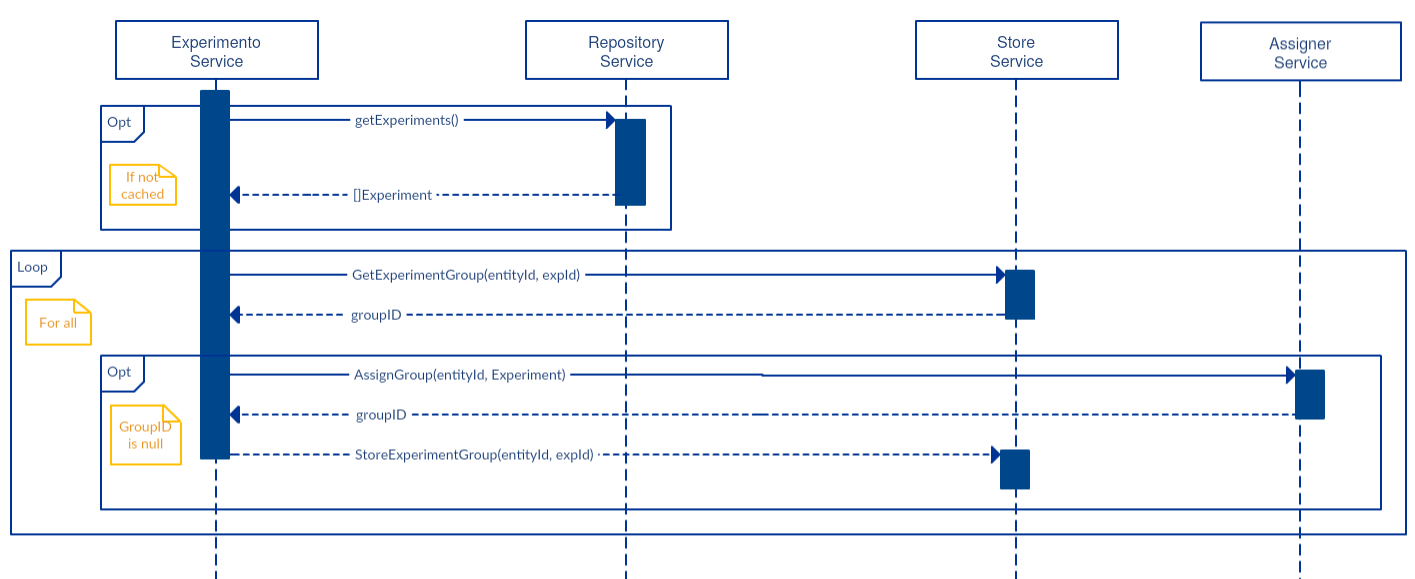
\includegraphics[max width=14cm,keepaspectratio]{sequence}
	\caption{Diagrama pentru modul de procesare a unei cereri}
	\label{fig:sequence}
\end{figure}

Vom detalia figura \ref{fig:sequence}, pentru a o complementa cu explicațiile necesare înțelegerii sistemului

\subsubsection{Obținerea experimentelor active}
Prima acțiune pe care serviciul \textit{Experimento} o va efectua este aceea de a verifica lista tuturor experimentelor. Acesta va avea implmentat local un mecanism de \textit{caching}, iar în cazul în care lista experimentelor se află în memorie, și \textit{cache-ul} nu a fost invalidat, serviciul va folosi această valoare. În caz contrar, se va efectua o cerere către serviciul \textit{Repository} și va aștepta răspunsul acesteia. 

\begin{remark}
	Modul de implementare al mecanismului de caching intră în atribuțiile microserviciului \textit{Experimento}.
\end{remark} 

\subsubsection{Verificarea asignării anterioare}

Este foarte important ca fiecare entitate să fie asociată constant către acelăși grup din cadrul unui experiment. După cum nu există nicio restricție asupra caracterului determinist al serviciului \textit{Assigner}, este necesară interogarea serivicului \textit{Store}. Acesta va răspunde cu un identificatorul unui grup, în cazul în care entitatea a fost anterior asignată, sau cu \textit{null} în caz contrar. 
Dacă entitatea are un grup deja asignat atunci acesta va fi rezultatul pe care cererea îl va furniza. 

\subsubsection{Asignarea unui grup}

Dacă la pasul anterior nu s-a găsit niciun grup ce a fost deja asignat experimentului, vom efectua o cerere către serviciul \textit{Assigner} prin intermediului interfeței descrise anterior. Acesta va răspunde cu identificatorul unui grup, pe care îl vom trimite pentru stocare apoi serviciului \textit{Store}. 

\begin{remark}
	Nu vom aștepta finalizarea apelului de stocare al experimentului, pentru a putea îmbunătăți performanța sistemului.
\end{remark}

Se poate observa cum pentru fiecare experiment în parte vom executa posibil ultimii doi pași descriși. Se vor compune apoi toate rezultatele corespunzătoare și va fi furnizat clientului rezultatul final al cererii.

În cazul în care se dorește aflarea variabilelor unei entități din cadrul unui singur experiment, modificările ce sunt necesare sunt imediate, iar lucrarea lasă cititorului ca exercițiu acest aspect.

\begin{remark}
	Iterațiile pentru determinarea grupului asignat unei entități pentru fiecare experiment, se vor exectua în mod \textit{concurent}. Acest lucru va îmbunătăți semnificativ performanța sistemului.
\end{remark}

\section{Concluzii}

În finalul acestui capitol, vom recapitula toate aspectele importante identificate pe parcursul acestuia. Așadar, vom folosi arhitectura bazată pe \textit{microservicii} pentru construcția serviciului de experimentare pe care lucrarea îl propune, acest fapt fiind datorat în special extensibilității și flexibilității pe care o are un astfel de sistem.

Apoi, am indetificat 4 servicii majore ce vor trebui implementate: \textit{Experimento}, serviciul central, \textit{Assigner}, serviciul responsabil cu asignarea identificatorilor către un grup, \textit{Store}, serviciul responsabil cu salvarea asignărilor, și \textit{Repository}, serviciul ce va gestiona lista experimentelor. Lucrarea a prezentat apoi o serie de mesaje ce vor acționa ca primitive în comunicările ce vor avea loc între servicii. Prin standardizarea structurii mesajelor, se obține o structură principală vitală pentru un serviciu ce propune un grad de extensibilitate foarte mare. Nu în ultimul rând am definit câte o interfață, pentru fiecare din microservicii, ce vor trebui să fie implementate, alături de descrierea generală a sistemului. 

Am ilustrat astfel toate elementele necesare construcției unui sistem de experimentare. Nu in ultimul rând trebuie făcută observația că singura componentă ce influențează efectele unui experiment este cea de \textit{Assigner}. De aceea, în următorul capitol, vom analiza posibilele strategii pentru a minimiza efectele negative ale unui experiment, maximizând deopotrivă aspectele pozitive ale acestuia.